\documentclass[a4paper,12pt]{article}
\usepackage{../../mypackages}
\usepackage{../../macros}

\setlength{\parindent}{0pt}


\begin{document}

\title{Chapitre 6 - Forces et intéractions}
\author{N. Bancel}
\date{Janvier 2025}
\maketitle

\section*{Effet d'une action sur le mouvement d'un corps}

\begin{compactitem}
  \item Une action s'exerçant sur un corps entraîne une \textcolor{blue}{modification de son mouvement ou une mise en mouvement}
  \item Deux corps sont en \textcolor{blue}{interaction} si le mouvement de l'un dépend de la présence de l'autre.
  \item Une \textcolor{blue}{action de contact} ne peut exister qu'entre deux corps en contact l'un avec l'autre. 
  \item Une action entre deux corps est une \textcolor{blue}{action à distance} lorsqu'il n'y pas de contact entre eux.
\end{compactitem}

\vspace{20em}


\subsection*{Classification}

Placer dans le tableau les actions listées ci-dessous : 

\begin{enumerate}[noitemsep]
  \item Force gravitationnelle exercée par la Terre sur un objet (appelée Poids)
  \item Tenir un livre dans la main
  \item Force d'attraction d'un aimant
  \item Action exercée par une règle en plastique sur des morceaux de papier (après avoir été frottée avec un tissu sec)
  \item Punaise enfoncée dans une planche
  \item Action du vent sur la voile d'un bateau
  \item Poussée d'un moteur sur un avion
\end{enumerate}

  \begin{center}
    \renewcommand{\arraystretch}{2} % Adjusts the row height
    \begin{tabularx}{\textwidth}{|>{\centering\arraybackslash}X|>{\centering\arraybackslash}X|}
      \hline
      \textbf{Action de contact} & \textbf{Action à distance (Répartie ? Ponctuelle ?)} \\
      \hline
      \rule{0pt}{16em} & \rule{0pt}{16em} \\ % Adds vertical space in cells
      \hline
    \end{tabularx}
  \end{center}

  \subsection*{Diagramme objet intéractions}

  \vspace{10em}


  \begin{tcolorbox}[colback=green!10!white, colframe=green!75!black, title=Méthode]
    \begin{compactitem}
      \item Identifier le système étudié. Le placer au centre du diagramme
      \item Identifier les objets susceptibles d'interagir avec lui. Les placer autour du système 
      \item Représenter les interactions
    \end{compactitem}
  \end{tcolorbox}

  \subsection*{Exemple}

  \begin{figure}[H]
    \centering
    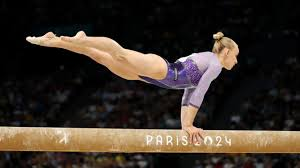
\includegraphics[width=0.6\linewidth]{img/cours_corps_03.jpeg}
    \caption{\label{} Athlète}
  \end{figure}

  Représenter le diagramme objet-intéraction de l'athlète

  \vspace{10em}

\subsection*{Exercices}

\subsubsection*{Exercice 1}

\begin{figure}[H]
  \centering
  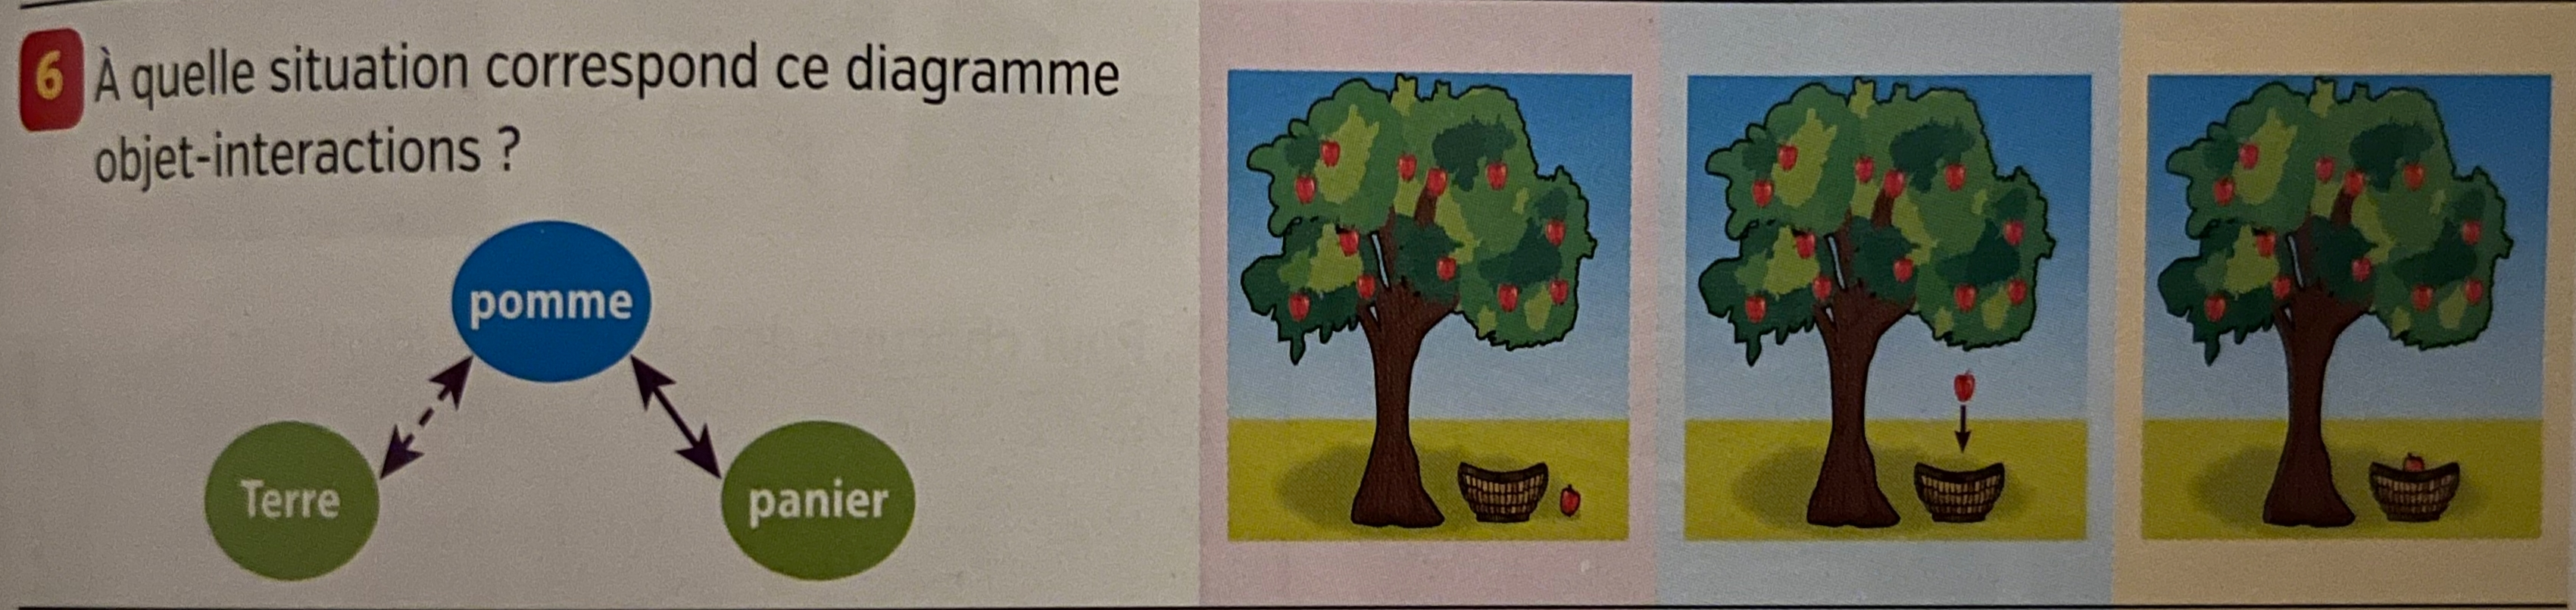
\includegraphics[width=0.9\linewidth]{img/cours_corps_02.jpg}
  \caption{\label{} Pomme}
\end{figure}

Dessiner les diagrammes objet-intéractions des 2 autres situations

\subsubsection*{Exercice 2}

Dessiner le diagramme objet-intéractions d'une bille en acier qui roule sur le sol et qui est attirée par un aimant ?

\section*{Modélisation d'une intéraction par une force}

\begin{tcolorbox}[colback=green!10!white, colframe=green!75!black, title=Méthode]
  Une intéraction est modélisée par une force représentée à l'aide d'une flèche dont la longueur est proportionnelle à la valeur de la force. \par 
  \vspace{1em}
  Une force est définie par 
  \begin{compactitem}
    \item 
    \item 
    \item 
    \item 
  \end{compactitem}
  \vspace{1em}
  L'unité d'une force est le \textcolor{blue}{Newton} et est notée $N$
\end{tcolorbox}

\begin{figure}[H]
  \centering
  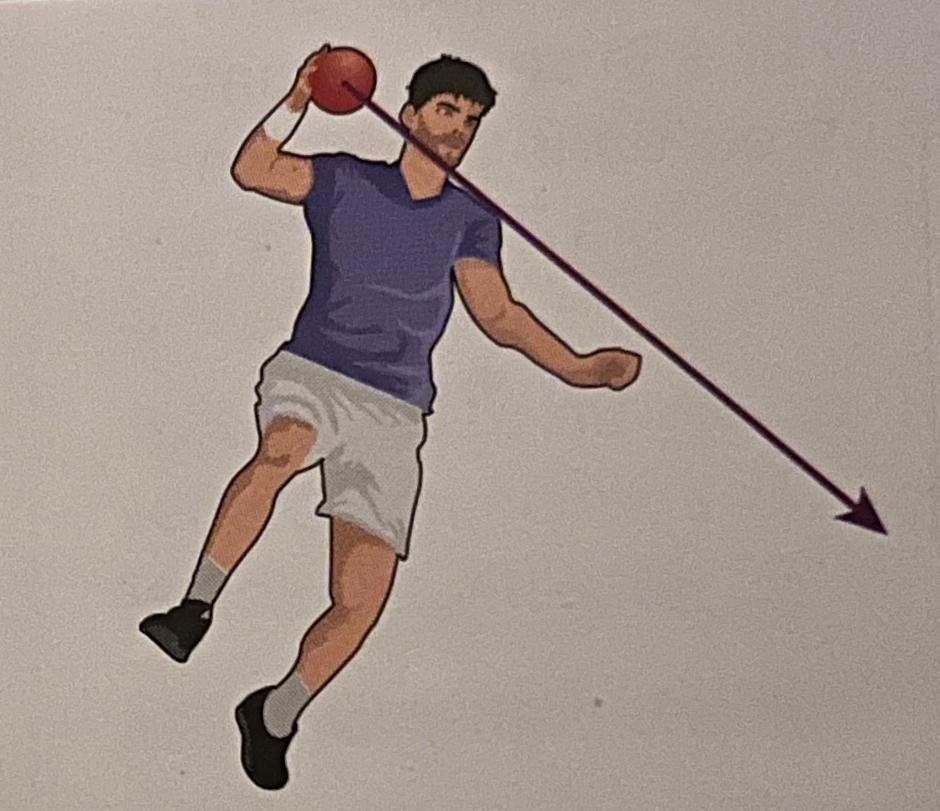
\includegraphics[width=0.5\linewidth]{img/cours_corps_04.jpg}
  \caption{\label{} Intéraction entre un handballeur et son ballon}
\end{figure}

\begin{compactitem}
  \item Direction : 
  \item Sens : 
  \item Point d'application : 
  \item Valeur : 100 Newtons
\end{compactitem}

\subsection*{Exercices}

\begin{figure}[H]
  \centering
  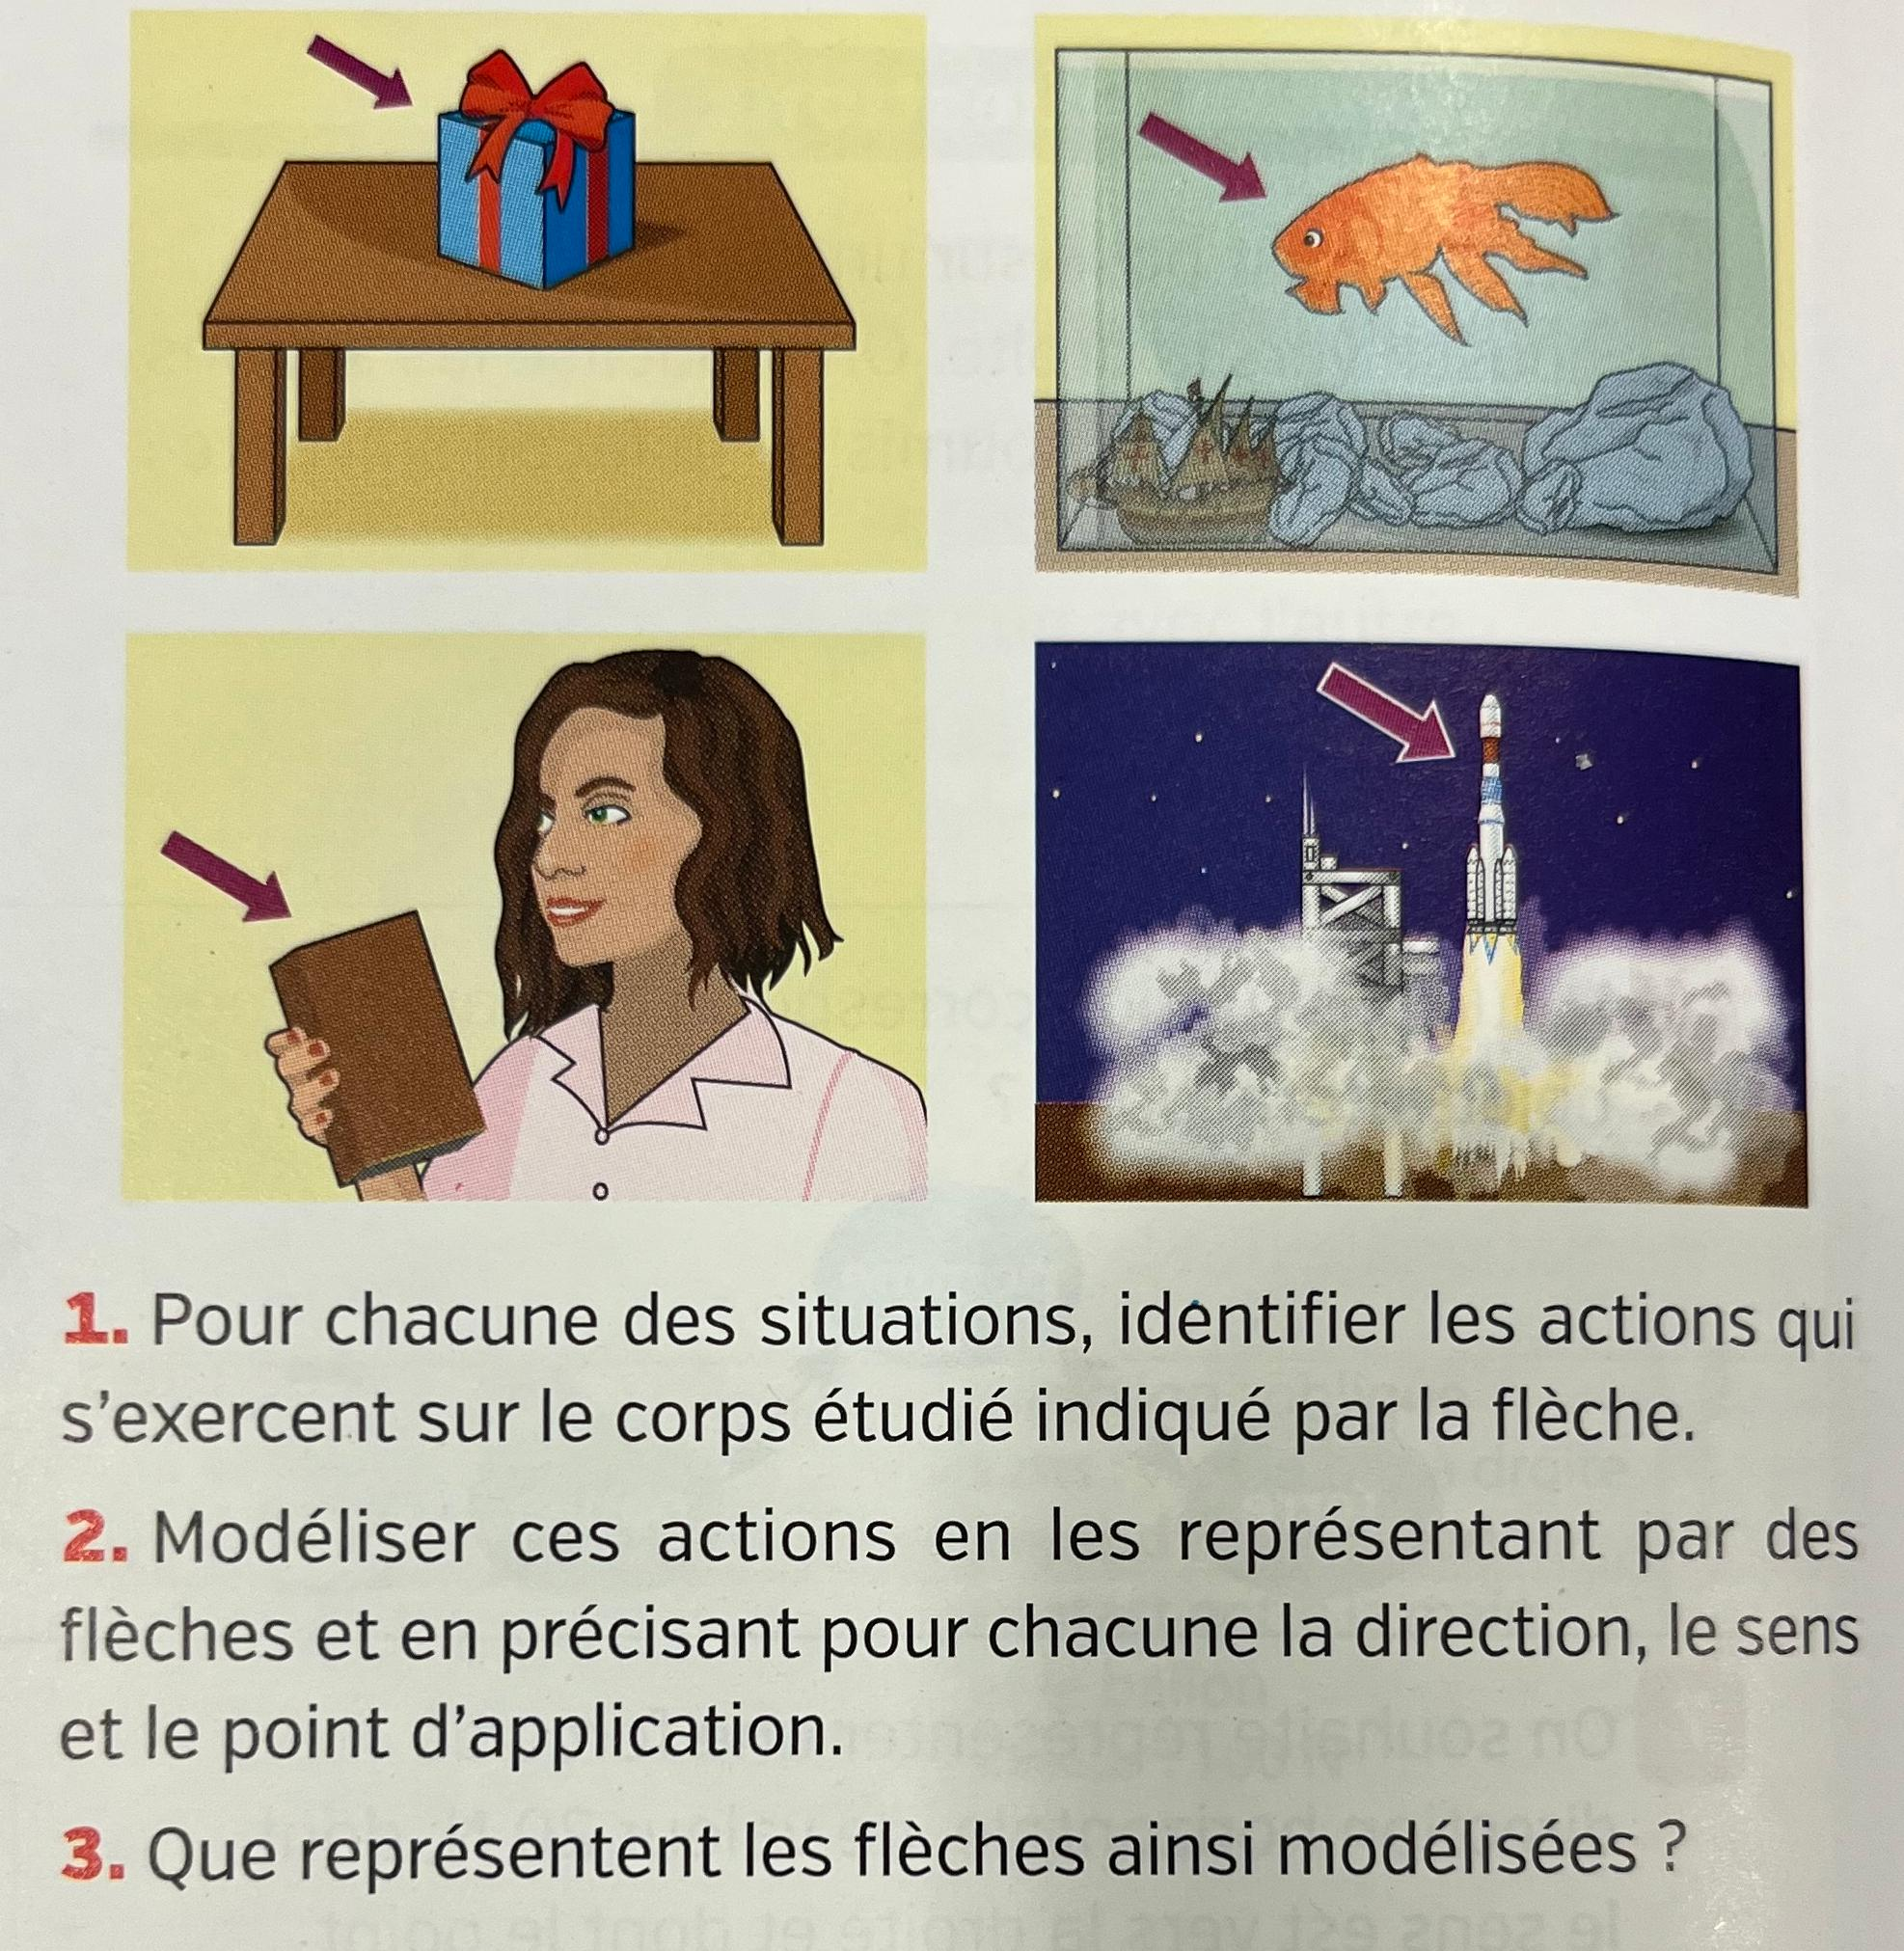
\includegraphics[width=0.7\linewidth]{img/cours_corps_05.jpg}
  \caption{\label{} Exercice 1 - Forces}
\end{figure}


\begin{figure}[H]
  \centering
  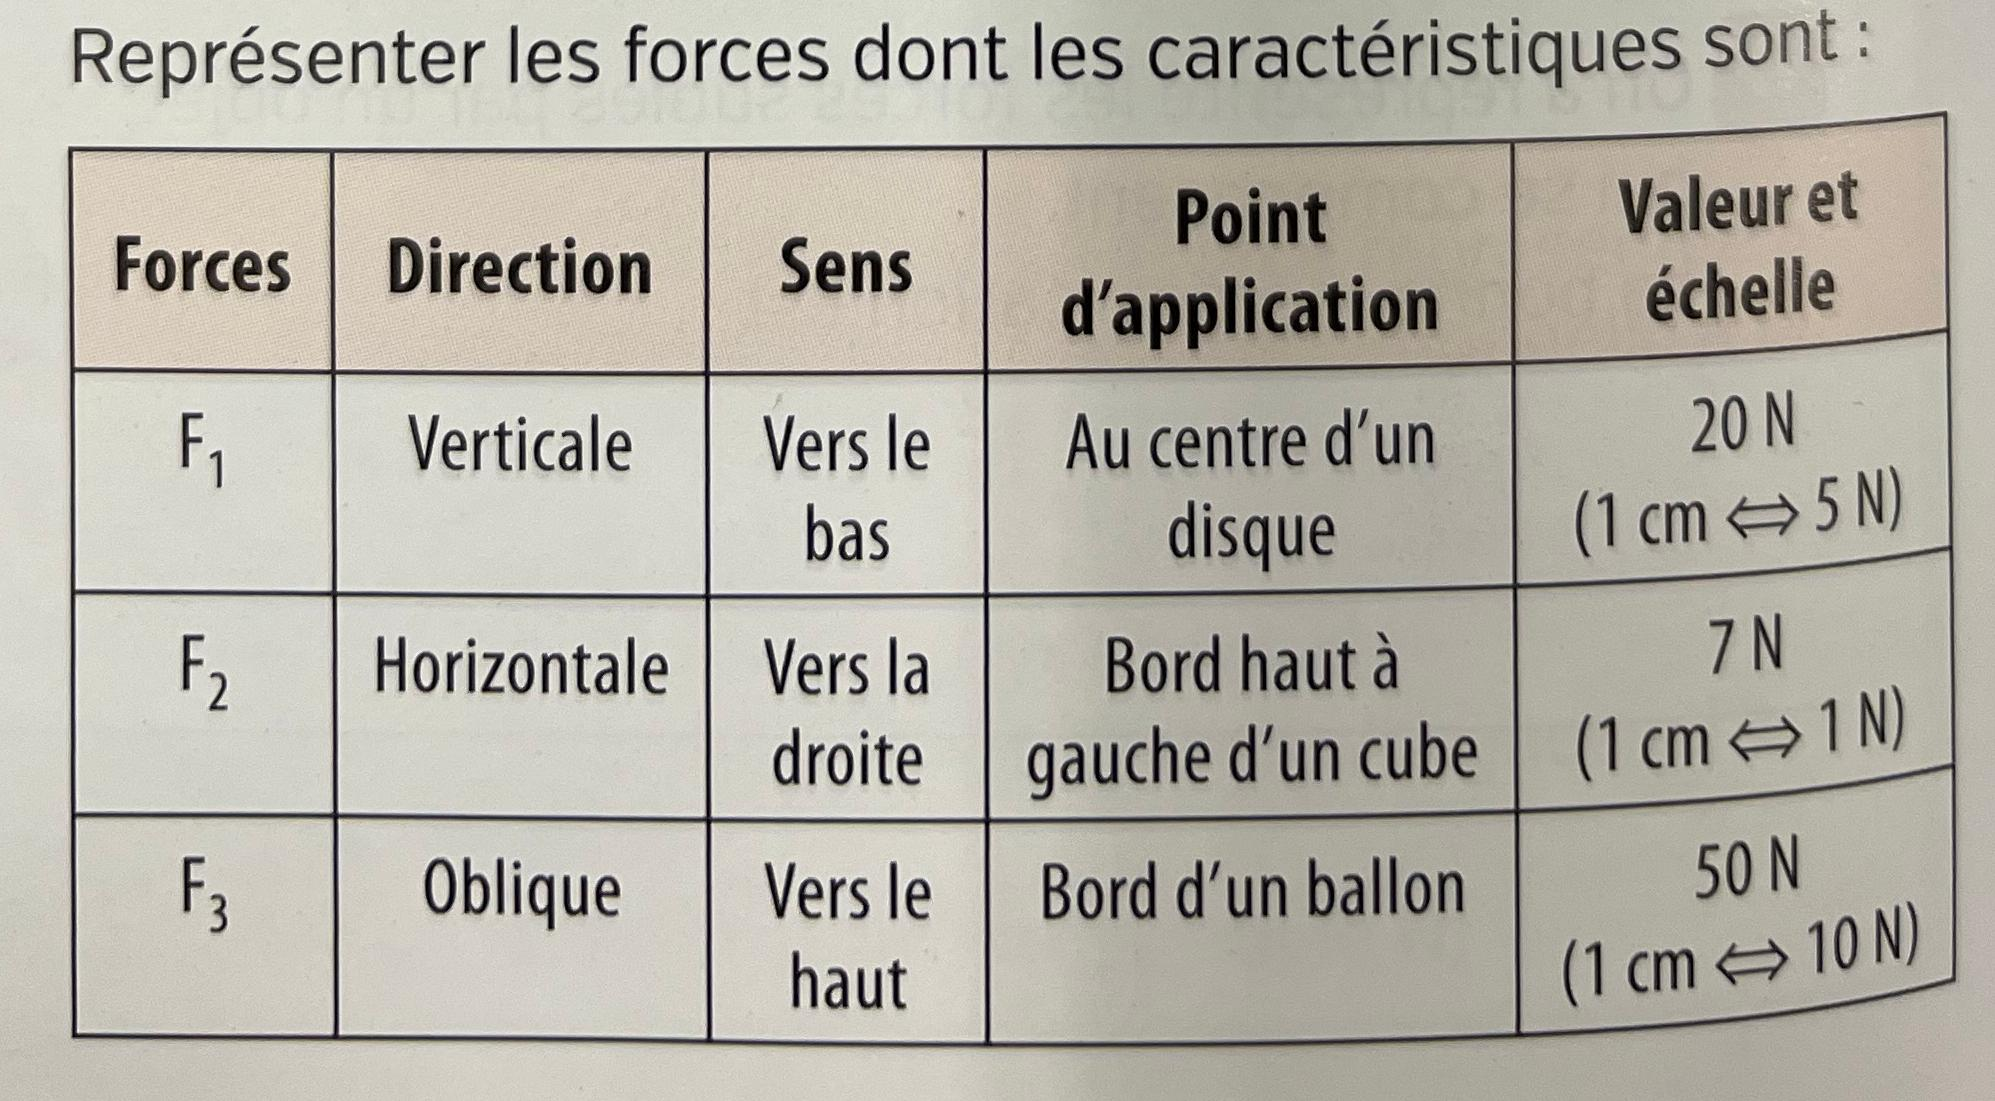
\includegraphics[width=0.7\linewidth]{img/cours_corps_06.jpg}
  \caption{\label{} Exercice 2 - Forces}
\end{figure}

\section*{Le principe d'inertie}

\begin{tcolorbox}[colback=green!10!white, colframe=green!75!black, title=Principe d'inertie]
  \textbf{Définition préalable :} On dit que deux forces (représentées par des vecteurs) se compensent si elles ont la même direction, des sens opposés, et la même valeur. \par
  \vspace{15em}
\end{tcolorbox}

\textbf{Exemples : }
\begin{itemize}
\item Mouvement d'un palet de air hockey ?
\vspace{3em}
\item Mouvement des planètes dans le référentiel héliocentrique ?
\vspace{3em}
\end{itemize}

\begin{figure}[H]
  \centering
  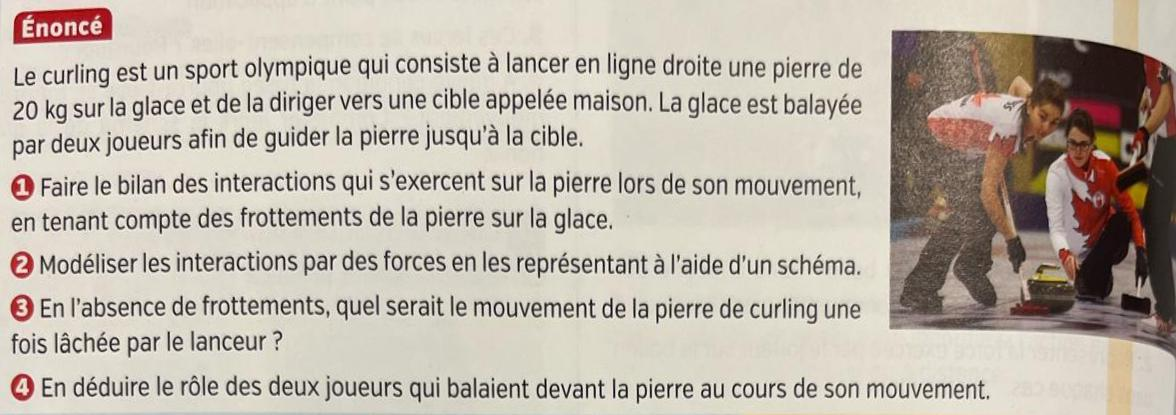
\includegraphics[width=0.8\linewidth]{img/cours_corps_07.jpg}
  \caption{\label{} Exercice 3 - Forces}
\end{figure}


\begin{figure}[H]
  \centering
  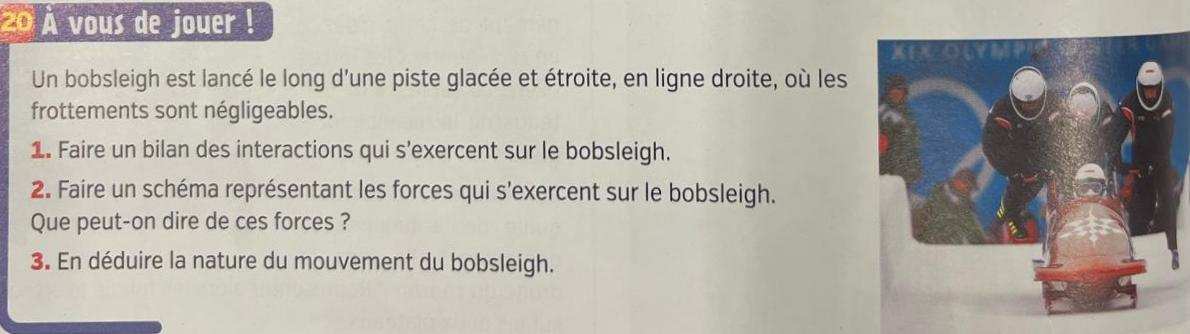
\includegraphics[width=0.8\linewidth]{img/cours_corps_08.jpg}
  \caption{\label{} Exercice 4 - Forces}
\end{figure}

\end{document}
